\section{Models for quantitative predictors}\label{sec:logist-quant}
Logistic regression models may use quantitative predictors or discrete
predictors, or a mixture of both, just as in ordinary regression models.
We describe the basic theory and visualization steps for
quantitative predictors here, and extend these ideas to discrete
explanatory variables in \secref{sec:logist-qual}.

\subsection{Fitting logistic regression models}
The parameters in logistic regression models are usually estimated
by maximum likelihood.
Because the response variable, $Y$, takes on only two values, we may
take these as 
1 and 0 with probabilities
$\pi$ and $1-\pi$, respectively.  Then
the probability distribution for case $i$ can be represented
simply as
\begin{equation*}
 p ( y_i ) \equiv \Pr (Y_i = y_i) = {\pi_i}^{y_i} \: (1 - \pi_i)^{1 - y_i}
 \period
\end{equation*}
Assuming the cases are independent, the joint probability of
the $n$ observations $y_1 , y_2 , \dots , y_n$ is the
product of these probabilities over all cases,
\begin{equation*}%\label{eq:like2}
p ( y_1 , y_2 , \dots , y_n ) = \prod_{i=1}^n {\pi_i}^{y_i} \: (1 - \pi_i)^{1 - y_i}
 = \prod_{i=1}^n {\left( \frac{\pi_i}{1 - \pi_i} \right)}^{y_i} (1 - \pi_i)
 \period
\end{equation*}
Substituting for $\pi_i$ from \eqref{eq:logit3},
we can express the likelihood of the data
as a function of the model parameters,
\begin{equation}\label{eq:like3}
\mathcal{L}(\alpha, \beta) =
 \prod_{i=1}^n [ \exp( \alpha + \beta X_i ) ]^{y_i} [1 + \exp( \alpha + \beta X_i )]^{-1} \period
\end{equation}
The maximum likelihood estimates are the values of $\alpha$ and $\beta$
which maximize $ \mathcal{L}(\alpha, \beta)$,
but it is simpler to maximize $\log \mathcal{L}$,
which has its maximum at the same values.
Taking derivatives of $\log \mathcal{L}$
with respect to $\alpha$ and $\beta$
gives the estimating equations (in matrix form)
\begin{equation}\label{eq:like4}
\mat{X} \trans \vec{y} = \mat{X} \trans \hat{\vec{p}}
\comma
\end{equation}
where $ \mat{X} = [ \vec{1}, \vec{x} ]$,
and
$\hat{p_i} = \exp (\hat{\alpha} + \hat{\beta} x_i) / (1+ \exp (\hat{\alpha} + \hat{\beta} x_i) $.
This is analogous to the linear model estimating equations in
ordinary least squares regression,
$\mat{X} \trans \vec{y} = \mat{X} \trans \hat{\vec{y}}$,
where $\hat{\vec{y}} = \mat{X} \hat{\vec{\beta}}$,
and $ \hat{\vec{\beta}} =  (\mat{X} \trans \mat{X})^{-1}  \mat{X} \trans \vec{y}$.
The equations \eqref{eq:like4} have no analytic solution, but they may be solved numerically, or by iteratively
reweighted least squares.

\begin{Example}[arthrit6a]{Arthritis treatment}
It is also straight-forward to calculate the values of $\log \mathcal{L}$
in \eqref{eq:like3}
for a grid of values of $(\alpha$ , $\beta)$
and plot the log likelihood surface as a contour plot or 3D plot.
For example, the \Dstp\ below calculates the log likelihoods
over all observations in the arthritis data
for a range of $\alpha$ (\pname{b0}) and $\beta$ (\pname{b1})
determined from the parameter estimates $\pm$ two standard errors
found in \exref{ex:arthrit7}
(see \outref{out:logist1c.1}).
The contour plot, shown in \figref{fig:likefun}, has its maximum
value $\log \mathcal{L} = -54.58$ at the value
$(\hat{\alpha} , \hat{\beta}) = (-2.64, 0.05)$.  From this,
$-2 \log \mathcal{L} = 109.16$ is the value displayed for \pname{-2 LOG L} in
\outref{out:logist1c.1} for the intercept and covariates.
%% one figure
\begin{figure}[htb]
  \centering
  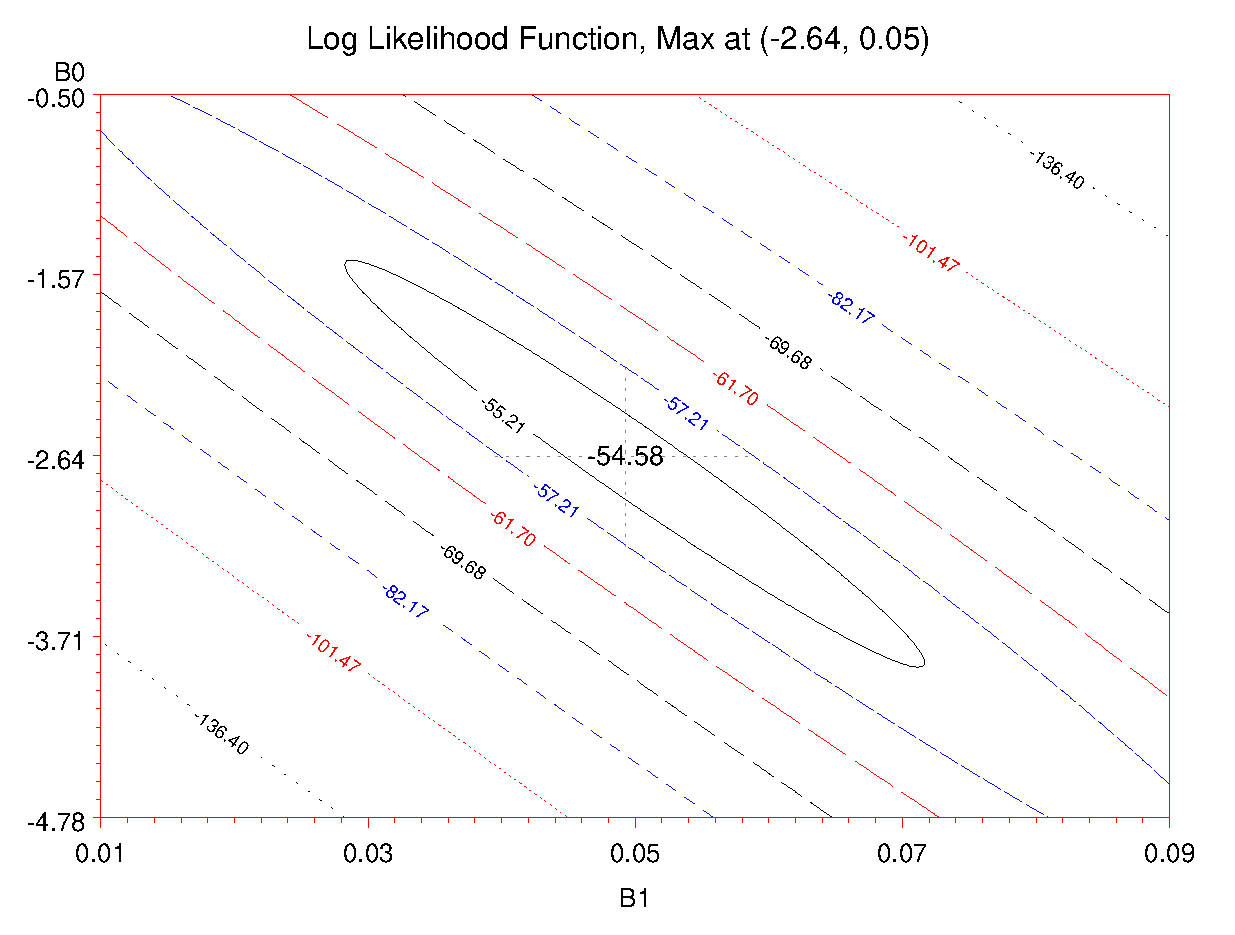
\includegraphics[clip,scale=.6]{ch6/fig/likefun}
  \caption{Contour plot of log likelihood for the Arthritis data}%
  \label{fig:likefun}
\end{figure}

\begin{listing}
data maxlike;
   keep b0 b1 loglike;
   do b0=(-2.64 - 2*1.07) to (-2.64 + 2*1.07) by (1.07/50);
      do b1=(0.05 - 2*0.02) to (0.05 + 2*0.02) by (0.02/50);
         loglike=0;
         do i=1 to n;
            set arthrit point=i nobs=n;
            phat = exp(b0+b1*age)/(1+exp(b0+b1*age));
            loglike = loglike + (better * log(phat))
                                  + ((1-better) * log(1-phat));
            end;
         output;
         end;
      end;
   stop;
\end{listing}
This contour plot of the log likelihood function shows something that
is not apparent from the usual printed output:
The contours of equal log likelihood have a pronounced negative slope,
so an increase in $\beta$ may be compensated for by a decrease in 
$\alpha$ without changing the value of $\log \mathcal{L}$ appreciably.
As well, the innermost ellipse (corresponding to the largest absolute
contour value) is relatively wide along its major axis,
reflecting the fact that the precision of these estimates is not
extremely high.   Increasing the sample size would result in tighter
estimates of the slope and intercept.
This is the visual representation of the information presented in the
covariance matrix of the parameter estimates.
\end{Example}

Logistic regression models can be fit using \PROC{LOGISTIC}, \PROC{CATMOD},
\PROC{GENMOD} and \INSIGHT.  The examples in this chapter mainly
illustrate 
the use of \PROC{LOGISTIC} because it provides the widest range of
diagnostics and other facilities for these models.
  
The input \Dset\ for \PROC{LOGISTIC} can
be in one of three forms:
\begin{description}
\item[frequency form] is used with grouped data, as in a contingency table.
For a binary response,
there are two observations per group corresponding to the levels
of the response, and a variable containing the frequency for that
group.  A \stmt{FREQ}{LOGISTIC} is used to provide the frequency
variable.

\item[events/trial form] is also used with grouped binomial data.
There is one observation per group; one variable gives the number of
events and a second variable gives the number of trials.
A \stmt{FREQ}{LOGISTIC} is also used in this situation.

\item[case form] is used when there is one observation per case.
This form  is usually required when there are quantitative predictors.
\end{description}

\subsection{Plotting predicted probabilities}\label{sec:logist-quantp}
\PROC{LOGISTIC} calculates
predicted logits \eqref{eq:logit1}
and 
predicted probabilities \eqref{eq:logit3}
for each observation.
These results may be saved in an \ODS, from which plots
can be made.  The plots, often supplemented by standard errors or
confidence bands for these predictions, provide a visual means to
interpret the prediction equations.


\begin{Example}[arthrit7]{Arthritis treatment}
This example illustrates the use of \PROC{LOGISTIC} to fit a logistic
regression model with a quantitative predictor.
It also describes the steps required
to plot the observed binary response together with fitted
probabilities and confidence intervals.
We use the arthritis treatment data, and describe how
\figref{fig:logist1c1} was produced.

The following \Dstp\ creates a \Dset\ in case form
named \pname{arthrit}.  The dichotomous response,
\pname{better} is created from the actual outcome
variable \pname{improve}, which has values 0, 1, 2
corresponding to none, some, or marked improvement.

\begin{listing}
data arthrit;
   input id treat$ sex$ age improve @@ ;
   better  = (improve > 0);            /* Dichotomous response    */
   _treat_ = (treat ='Treated') ;      /* Dummy var for treatment */
   _sex_   = (sex = 'Female');         /*           and sex       */
  cards ;
57 Treated Male   27 1   9 Placebo Male   37 0
46 Treated Male   29 0  14 Placebo Male   44 0
77 Treated Male   30 0  73 Placebo Male   50 0
  ... {\it (observations omitted)}
56 Treated Female 69 1  42 Placebo Female 66 0
43 Treated Female 70 1  15 Placebo Female 66 1
                        71 Placebo Female 68 1
                         1 Placebo Female 74 2
\end{listing}

By default, \PROC{LOGISTIC} orders the response
values in \emph{increasing} order, and sets up the model so that it is
predicting the probability of the \emph{smallest} ordered value,
Pr\{better=0\}.  This means it would be modeling the probability of No
improvement here.  
The \opt{descending}{LOGISTIC} (available with Version 6.08)
reverses this order, so that predicted results will be for
Pr\{better=1\}.

\begin{listing}
proc logistic nosimple descending;
   model  better = age / lackfit;
   output out=results p=predict l=lower u=upper;
\end{listing}
Alternatively, you can use the \opt{order}{LOGISTIC}, or
(with the default \pname{order=formatted})
you can create a user-format for the 0/1 values of the
response so that the first (smallest) formatted value corresponds
to the desired event.  In the format \pname{outcome} below, the value
``improved'' conveniently comes first alphabetically,
and so would be the predicted event.
\begin{listing}
proc format;
   value outcome 0 = 'not improved'
                 1 = 'improved';
proc logistic nosimple;
   format better outcome.;
   model  better = age / lackfit;
   output out=results p=predict l=lower u=upper;
\end{listing}
In the printed output
(\outref{out:logist1c.1}) the Response Profiles show that the response
values are ordered as desired.

\begin{Output}[htbp]
\caption{Arthritis treatment data: Logistic regression on age}\label{out:logist1c.1}
\small
\verbatiminput{ch6/out/logist1c.1}
\end{Output}
The \stmt{OUTPUT}{LOGISTIC} shown above
produces an \ODS\ (\pname{RESULTS}) containing the predicted probability of
improvement (\pname{PREDICT}) and 95\% confidence limits
(\pname{LOWER}, \pname{UPPER}) for these observations.
The first few observations from the \Dset\ \pname{RESULTS}
are shown in \outref{out:logist1c.2}.
There is one observation per case because the input data are in case form.

\begin{Output}[htb]
\caption{Arthritis treatment data: RESULTS \Dset\ (partial)}\label{out:logist1c.2}
\small
\verbatiminput{ch6/out/logist1c.2}
\end{Output}

The plot shown in \figref{fig:logist1c1} is produced
as an overlay plot by the
following \PROC{GPLOT} step.
Three \stmt{SYMBOL}{GPLOT}s are used to plot point symbols
for the observed response (\pname{BETTER}) and
interpolated lines for the
predicted probabilities of improvement and confidence limits.
The linear regression lines (and its confidence limits) in the figure are produced using
the \pname{INTERP=RLCLM} on the \pname{SYMBOL1} statement.
\begin{listing}
proc sort data=results;
   by age;
proc gplot data=results;
   plot better * age = 1
        predict * age = 2
        upper * age = 3
        lower * age = 3
        / frame overlay vaxis=axis1 vm=1 hm=1;
   axis1 label=(a=90) offset=(3) order=(0 to 1 by .2);
   symbol1 v=dot h=1.4 i=rlclm l=2 c=green ci=red;
   symbol2 v=none   i=join l=1  w=3 c=blue;
   symbol3 v=none   i=join l=20 w=3 c=blue;
   label better='Probability (Improved)';
   format better 4.1;
   title2  c=red 'Linear' c=black ' and ' c=blue 'Logit '
           c=black 'Regressions on Age';
run;
\end{listing}
The model fitting tests in \outref{out:logist1c.1}
(``Chi-Square for Covariates'' and the Wald test for \texttt{age})
test whether
age adds significantly to predicting outcome.
This is a different question than whether the model is adequate---usually
provided by a \glossterm{lack of fit test},
comparing the given model to the saturated model.
However,
with binary data in case form, the usual lack of fit tests
do not apply.
The \opt{lackfit}{LOGISTIC} on the \stmt{MODEL}{LOGISTIC}
requests a lack-of-fit test
\ix{lack-of-fit test}
proposed by \citet{HosmerLemeshow:89}.  This test divides subjects
into tenths based on their ordered predicted probabilities. It then computes a
\(\chi^2\) from the observed and expected frequencies in these 10 groups. 
The results from this test,
shown in \outref{out:logist1c.3} do not reject the fit of the simple
one-variable model;  however, the relatively small $p$-value suggests that the model
might be improved.
\begin{Output}[htbp]
\caption{Arthritis treatment data: Goodness-of-fit test}\label{out:logist1c.3}
\small
\verbatiminput{ch6/out/logist1c.3}
\end{Output}
\end{Example}

%\subsubsection{The \emph{Challenger} disaster}
\begin{Example}[nasa]{Challenger disaster}
\ixd{Challenger disaster|(}
\begin{changebar}
The space shuttle \emph{Challenger} exploded 73 seconds after take-off on
\end{changebar} 
January 28, 1986.
Subsequent investigation determined that the cause was failure of the O-ring
seals used to isolate the fuel supply from burning gases.
The story behind the \emph{Challenger} disaster is perhaps the most poignant
missed opportunity in the history of statistical graphics.
It may be heartbreaking to find out that some important information
was there, but the graph maker missed it.

Engineers from Morton Thiokol, manufacturers of the rocket motors,
had been worried about the effects of unseasonably cold weather
on the O-ring seals and recommended aborting the flight.
NASA staff analysed the data on the relation between ambient temperature
and the number of O-ring failures (out of 6), but they had excluded observations
where no O-rings failed,
believing that they were uninformative.
Unfortunately, those observations had occurred when the launch temperature
was relatively warm (\degree{65-80}F.) and were indeed informative.
The coldest temperature at any previous launch was \degree{53};  when \emph{Challenger} was launched on January 28,
the temperature was a frigid \degree{31}.

The data relating O-ring failures to temperature were depicted as in
\figref{fig:nasa0}, our candidate for the most misleading graph of history.
Examination of this graph seemed to indicate that there was no relation
between ambient temperature and failure.  Thus, the decision to launch
the \emph{Challenger} was made, in spite of the initial concerns
of the Morton Thiokol engineers.
\begin{figure}[htb]
  \centering
  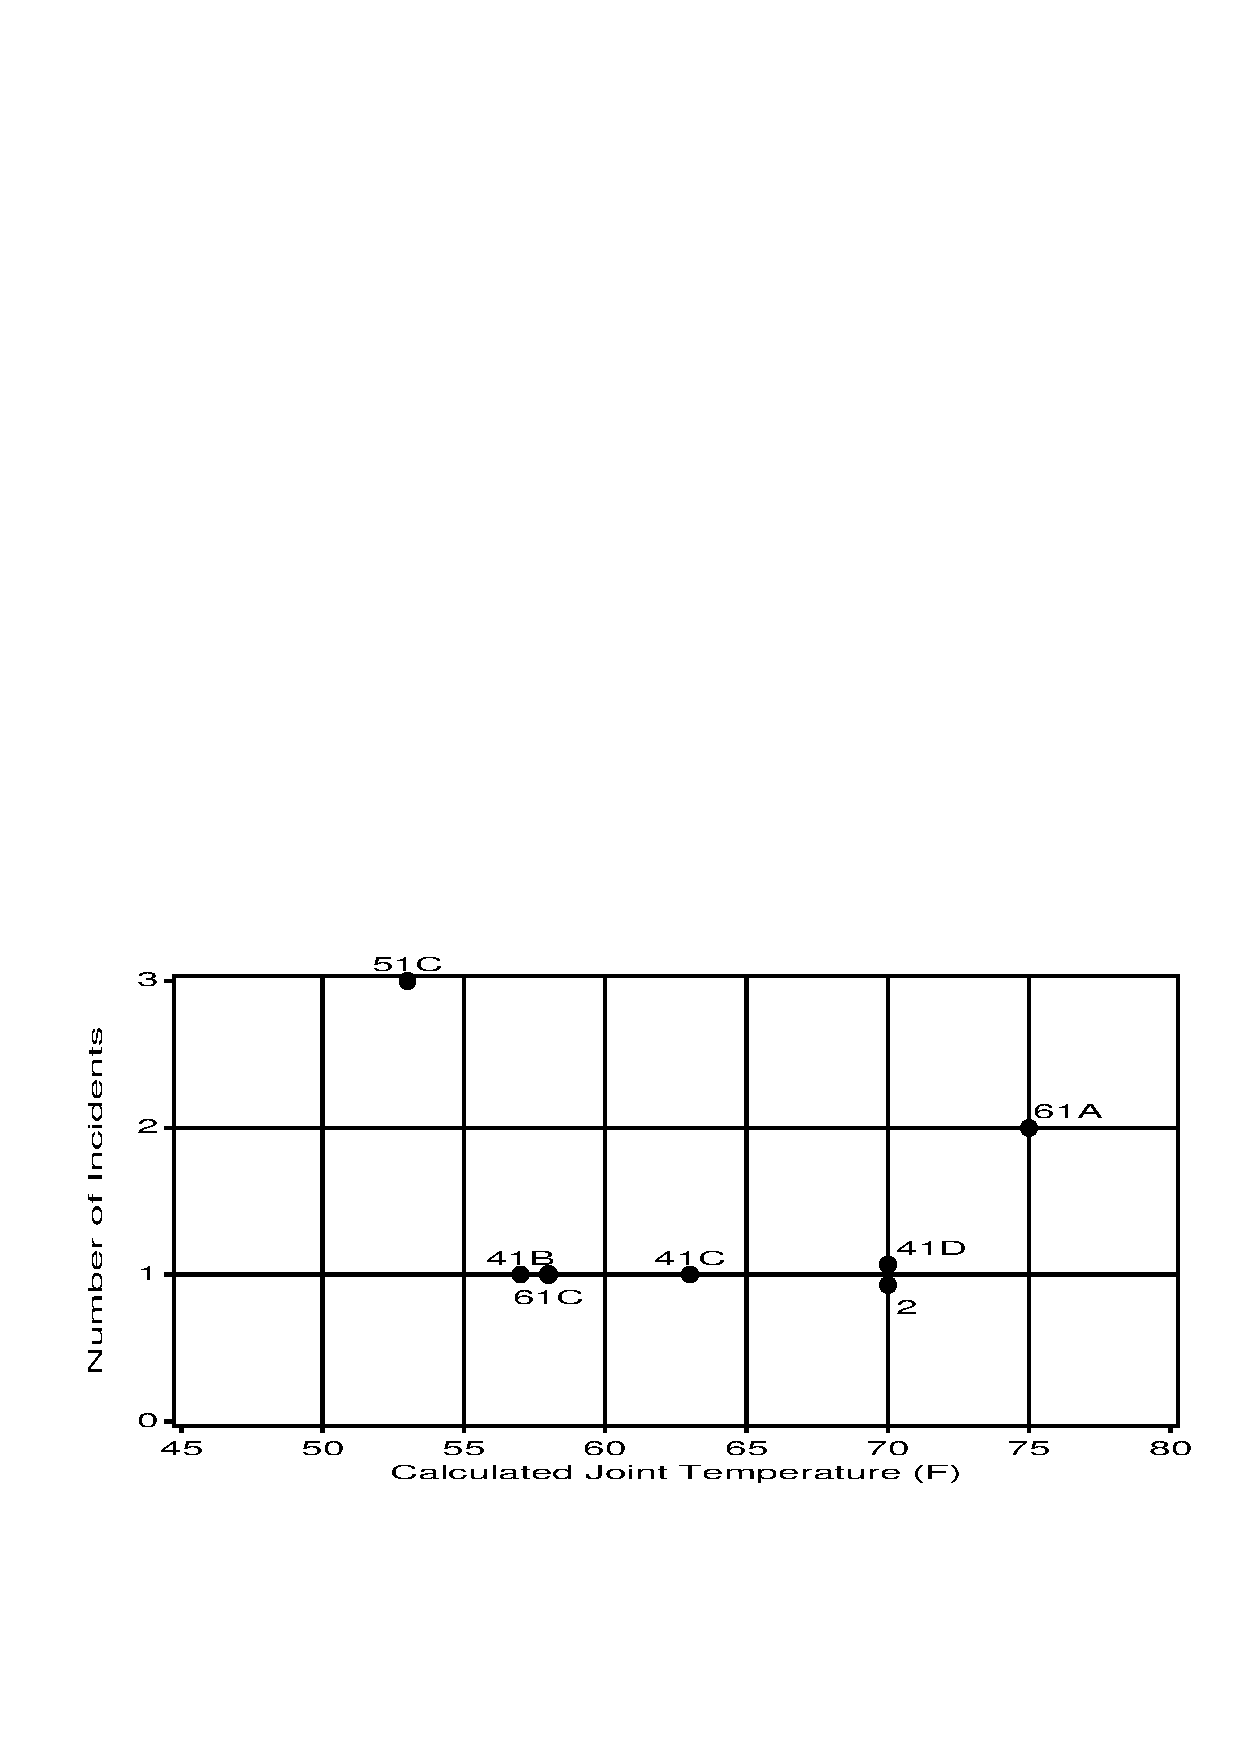
\includegraphics[width=\textwidth,clip]{ch6/fig/nasa0}
  \caption{NASA Space Shuttle pre-launch graph}\label{fig:nasa0}
\end{figure}

These data have been analyzed extensively
\citep{Dalal-etal:89,Lavine:91}.
\citet{Tufte:97} gives a thorough and convincing
visual analysis of the evidence available prior to the launch.
The main goal here is to
illustrate predictions from the model for the \emph{Challenger} launch
and graphical display.
But, what if the engineers had simply made a better graph?
At the least, that would entail
\begin{seriate}
\item drawing a smoothed curve to fit the points (to show the trend)
\item removing the background grid lines (which obscure the data).
\end{seriate}
\figref{fig:nasa02} 
shows a revised version of the same 
graph, which should have caused any engineer to conclude that
either 
\begin{seriate}
\item the data were wrong, or
\item there were excessive risks
associated with both high and low temperatures.
\end{seriate}
But it is well-known
that brittleness of the rubber used in the O-rings is inversely
proportional to $(\texttt{temp})^3$, so prudent interest might have focussed
on the first possibility.

\begin{figure}[htb]
  \centering
  \includegraphics[clip,width=\textwidth]{ch6/fig/nasa02}
  \caption{NASA Space Shuttle pre-launch graph, revised}\label{fig:nasa02}
\end{figure}

We return to the problem of predicting the likelihood of failures at
low temperatures.
The \Dstp{} below reads the data on the number of O-ring failures
and temperature for the 23 flights for which information was available
before the \emph{Challenger} launch.  A more detailed \Dset,
from \citet{Dalal-etal:89} and \citet{Tufte:97} is given in \datref{dat:orings}.

\begin{listing}
title 'NASA Space Shuttle O-Ring Failures';
data nasa;
   input failures temp @@;
   orings = 6;
   label failures = 'Number of O-ring failures'
      temp = 'Temperature (deg F)';
   datalines;
   2  53    1  57    1  58     1  63
   0  66    0  67    0  67     0  67
   0  68    0  69    0  70     0  70
   1  70    1  70    0  72     0  73
   0  75    2  75    0  76     0  76
   0  78    0  79    0  80
;
\end{listing}
To obtain predicted probabilities for observations not in the original sample,
create an additional \Dset\ which contains values for the independent
variables in the extrapolation sample, and join these observations to the
actual \Dset.  The response variable (\texttt{failures}) will be missing
for the extrapolation sample.

\begin{listing}
*-- Obtain predicted values for 30-80 degrees;
data temp;
   input temp @@;
datalines;
31 30 35 40 45 50 55 60 65 70 75 80
;
data nasa2;
   set nasa temp;
\end{listing}
In the \PROC{LOGISTIC} step, we use the \boldital{events/trials} syntax
to indicate the number of failures and number of trials.
(This does assume that O-rings on the same flight fail independently.)
The observations in the extrapolation sample are not used in fitting
the model, yet the procedure produces predicted probabilities and
logits (as long as the independent variable(s) are non-missing).

\begin{listing}
proc logistic data=nasa2 nosimple;
   model failures/orings = temp ;
   output out=results p=predict l=lower u=upper;
proc print;
\end{listing}
The printed output, shown in \outref{out:nasa.1} indicates that the
12 new observations were not used in the analysis.
The odds ratio, 0.891, is interpreted to mean that each increase of
\degree{1} in temperature decreases the odds of a failure by 11\%!

\begin{Output}[htbp]
\caption{Logistic regression for NASA O-ring data}\label{out:nasa.1}
\small
\verbatiminput{ch6/out/nasa.1}
\end{Output}

The \ODS\ \pname{results} contains the predicted probability
of a failure of a single O-ring
at each temperature and upper and lower confidence 95\% limits
for this probability.  We can plot the predicted and observed values
as shown below.  A vertical reference line at \degree{31} is used
to highlight the conditions at the \emph{Challenger} launch.
\begin{listing}
proc sort data=results;
   by predict;
data results;
   set results;
   obs = failures / orings;

proc gplot data=results;
   plot (obs predict lower upper) * temp /
      href=31 lhref=33
      overlay frame vaxis=axis1 vminor=1;
   symbol1 v=dot i=none c=blue h=2;
   symbol2 v=none i=spline c=black w=5;
   symbol3 v=none i=spline c=red l=33 r=2 w=3;
   axis1 label=(a=90 'Estimated Failure probability') offset=(3);
\end{listing}

The graph is shown in \figref{fig:nasa}.  There's hardly any data
at low temperatures and the width of the confidence band provides
an important visual cue to this uncertainty. Nevertheless,
the predicted probability of failure per O-ring is uncomfortably
 high at \emph{all} temperatures below the range of data from
previous flights.  Would you take a ride on \emph{Challenger} when
the weather is cold?

\begin{figure}[htb]
  \centering
  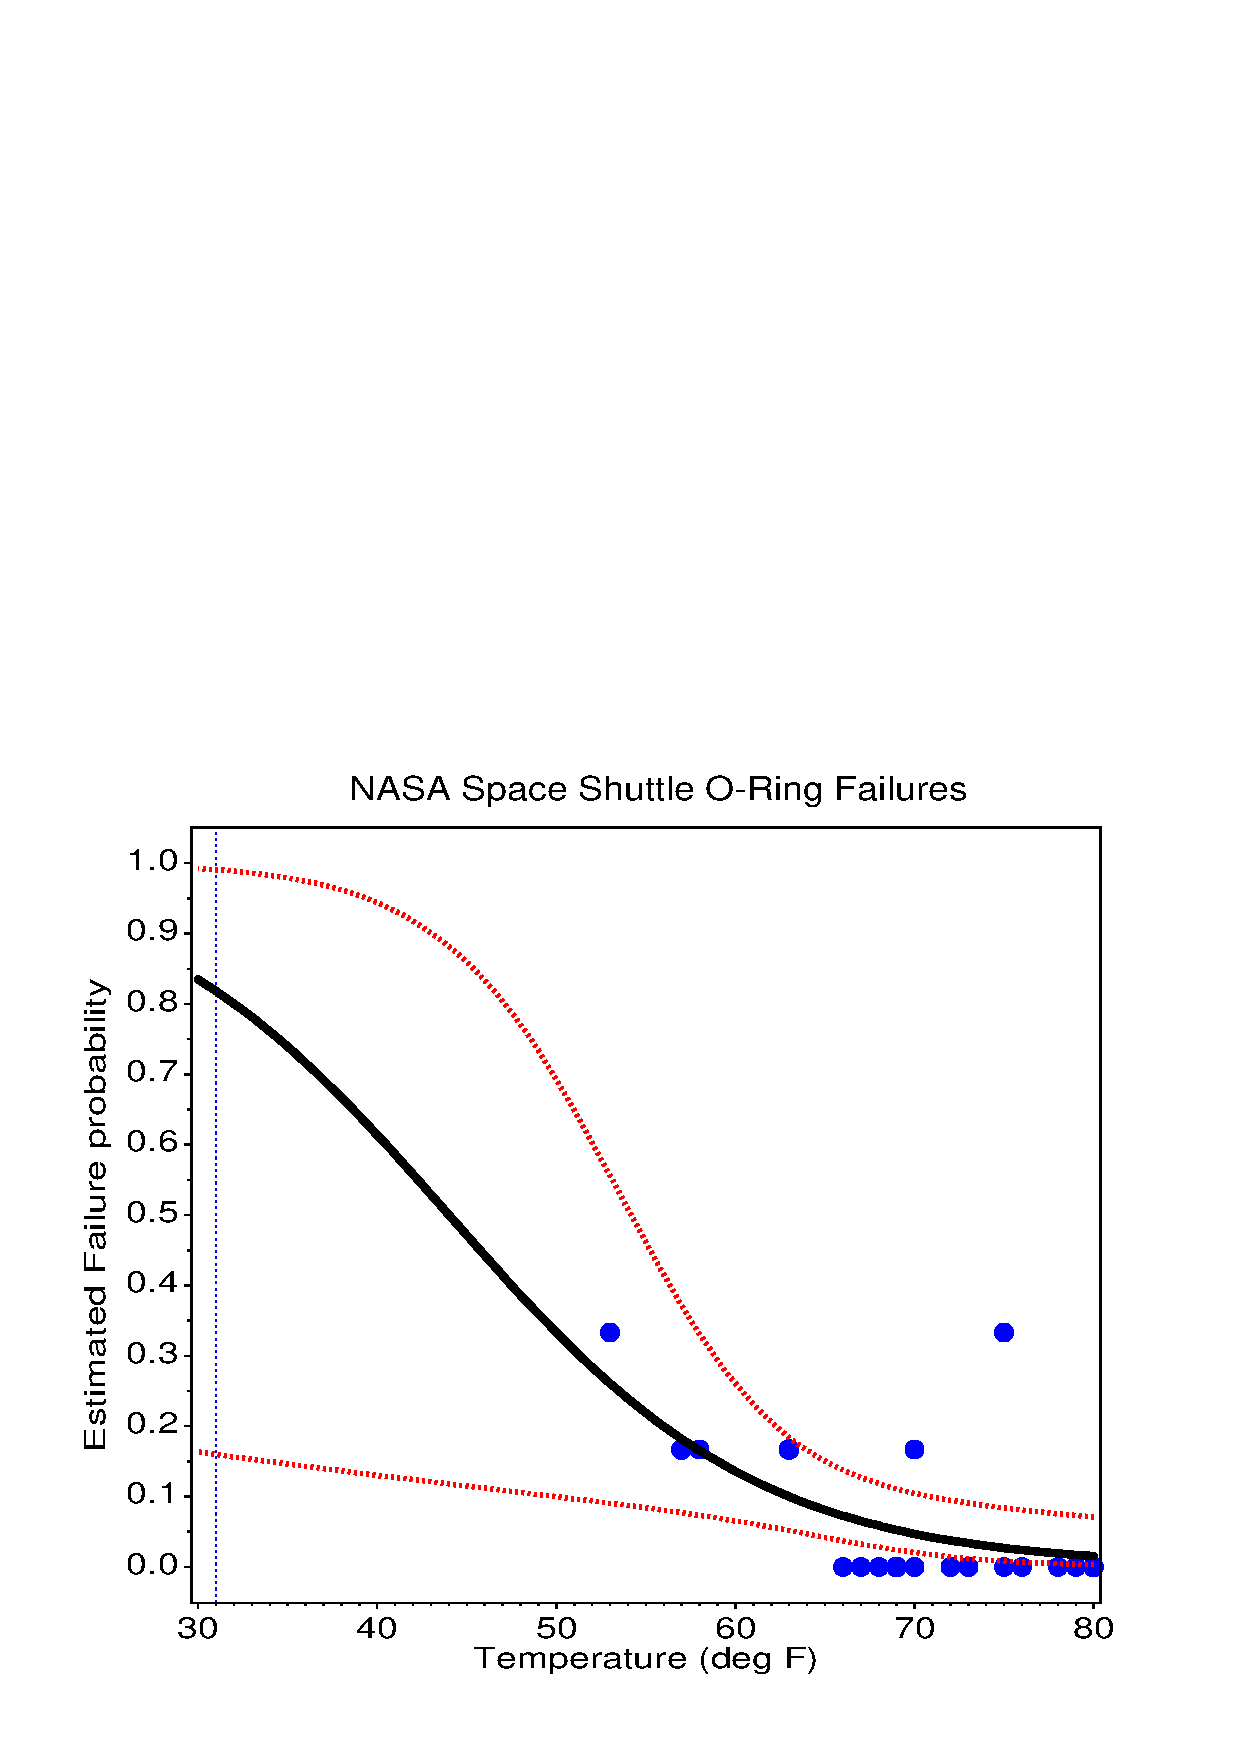
\includegraphics[scale=.75]{ch6/fig/nasa}
  \caption{NASA Space Shuttle O-ring Failure, Observed and Predicted probabilities}\label{fig:nasa}
\end{figure}
\ixd{Challenger disaster|)}
\end{Example}

